\chapter{Clases}
\section{Introducción}
Los diagramas de clase son parte importante del diseño de un software, ya que estos permiten generar diseños que plasmen la solución a un problema, la cual será entendible para todos aquellos conozan del lenguaje unificado de modelado (UML).
\\
Además es necesario utilizar diagramas de clase para representar gráficamente y de forma estática la estructura general del sistema, mostrando sus clases e interacciones.
\section{Teoría}
Los diagramas de clase sirven para visualizar las relaciones entre las clases que involucran el sistema,entre estas se encuentran:
\begin{itemize}
\item Dependencia.
\item Asociación.
\item Agregación.
\item Composición.
\item Generalización.
\item Realización.
\end{itemize}

Estas relaciones pueden subdividirse en dos grandes grupos: Las relaciones cliente/proveedor, en las cuales entran las dependencias y asociaciones (asociación, agregación y composición), las cuales generan un alto acoplamiento en el software, pero también lo hacen seguro. Por otro lado están las relaciones de generalizacion en las cuales están la especialización e implementacion. Estas poseen un bajo acoplamiento, pero no poseen la seguridad de las de cliente/proveedor. 
El ideal es crear un diagrama de clases en el que haya un equilibrio entre el acoplamiento y la seguridad.
\begin{figure}[H]
	\centering
	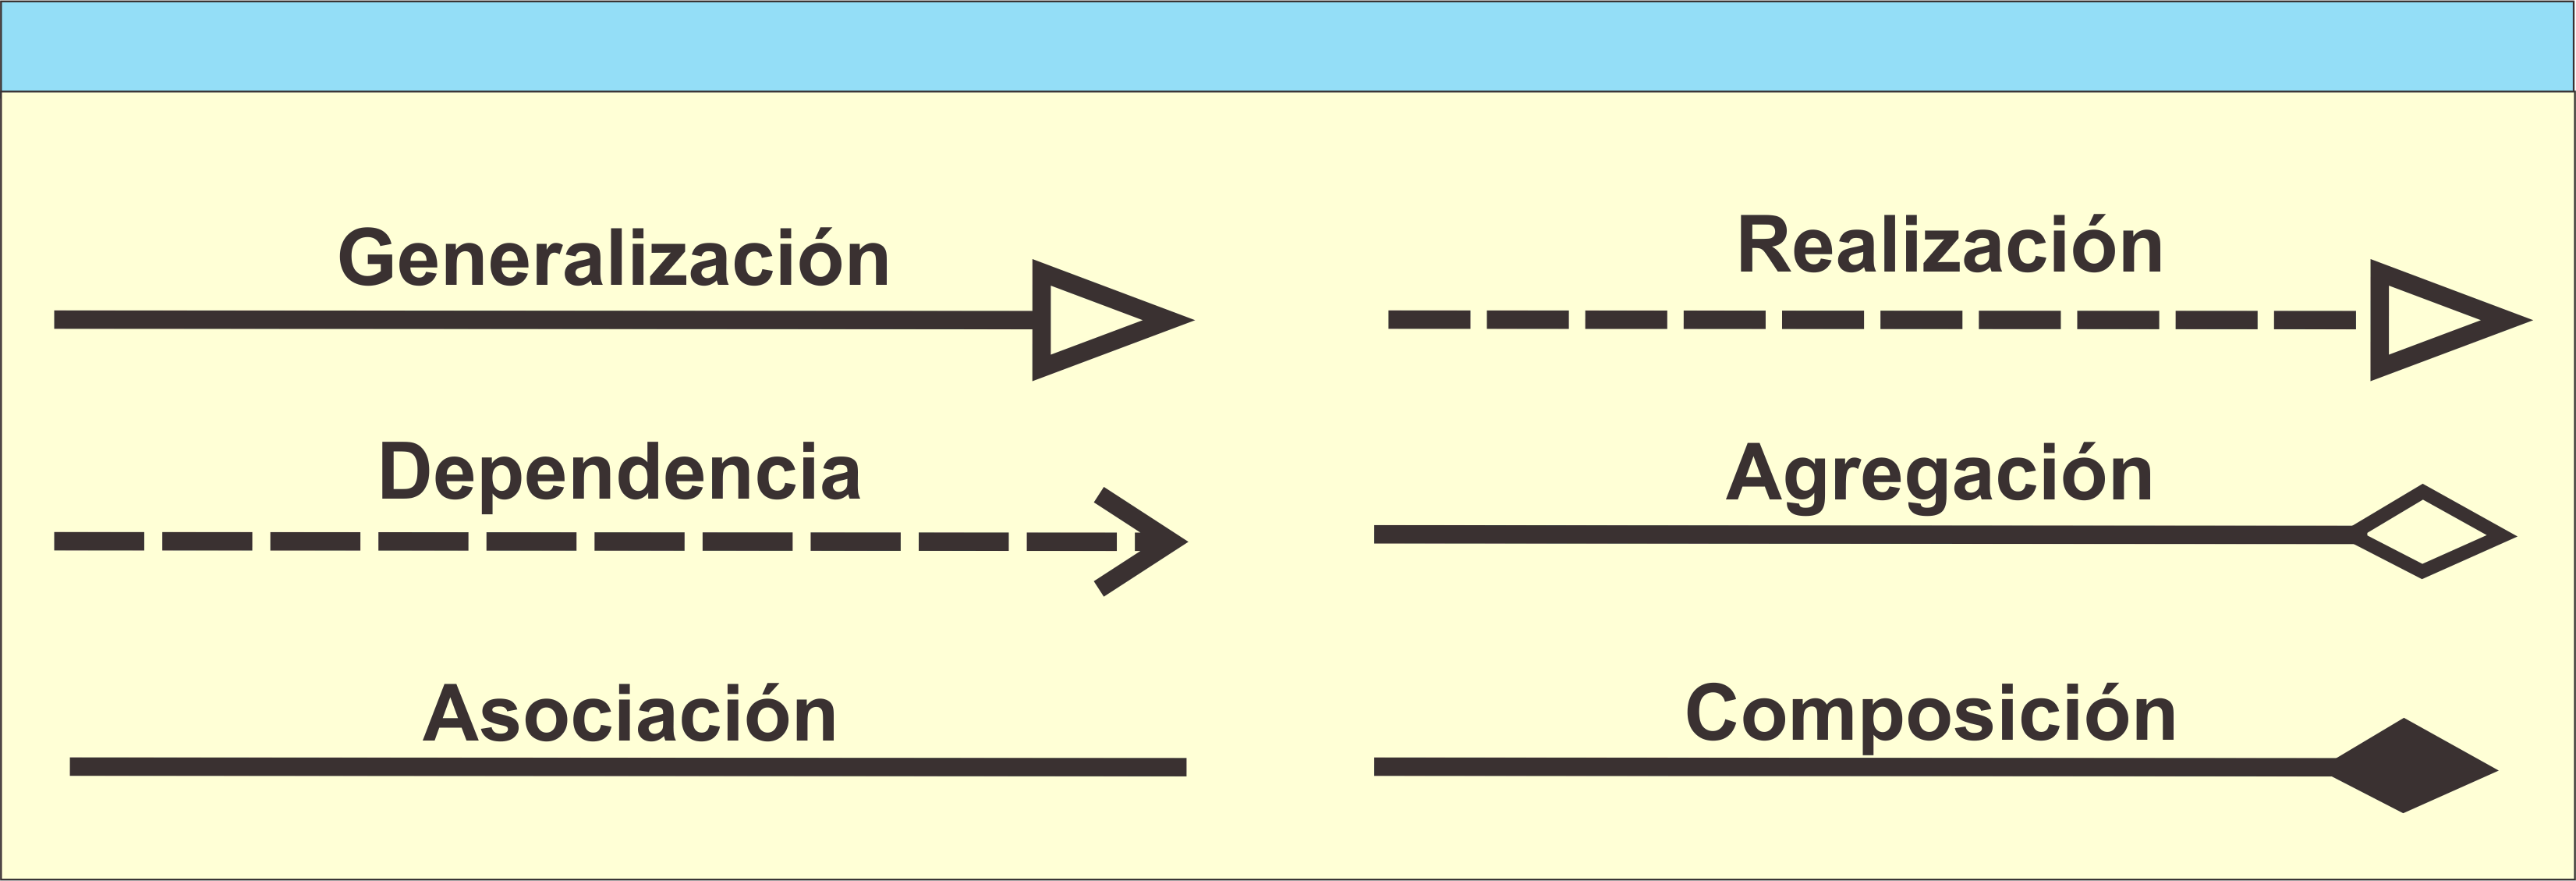
\includegraphics[width=1\linewidth]{diseno/clases/imagenes/relaciones.png}
	\caption{Relaciones UML. Tomada de internet}
	\label{fig:gantt}
\end{figure}
Por otro lado, las clases se representan por medio de un rectángulo que se divide en tres:
\begin{itemize}
\item Nombre de la clase: Cómo se denomina la clase. Es un sustantivo.
\item Atributos de la clase: Pueden ser de diferentes tipos (booleano, numérico, cadenas Y T.D.A), tienen modificadores de visibilidad (public, private, protected, de paquete), nombre y propiedades (final, const) si es necesario.
\item Métodos de la clase: Son las operaciones que realiza la clase, deben denominarse con verbos, poseen modificadores de visibilidad y pueden retornar diferentes tipos de datos (void, numérico, cadenas y T.D.A) Adicionalmente, los métodos pueden recibir argumentos, que se representan en las operaciones en forma de parámetros los cuales son variables que poseen nombre y tipo.
\end{itemize}
 